% ===================== QCD (adapted from the 2023 comprehensive-exam slides) =====================
\section{QCD}

% Slide 7
\begin{frame}{Quarks \& gluons}
  \quick
  \centering
  \textbf{Hadrons are made of more fundamental particles: quarks and gluons.}\\[2mm]
  \begin{columns}[c]
    \begin{column}{0.5\textwidth}
      \centering
      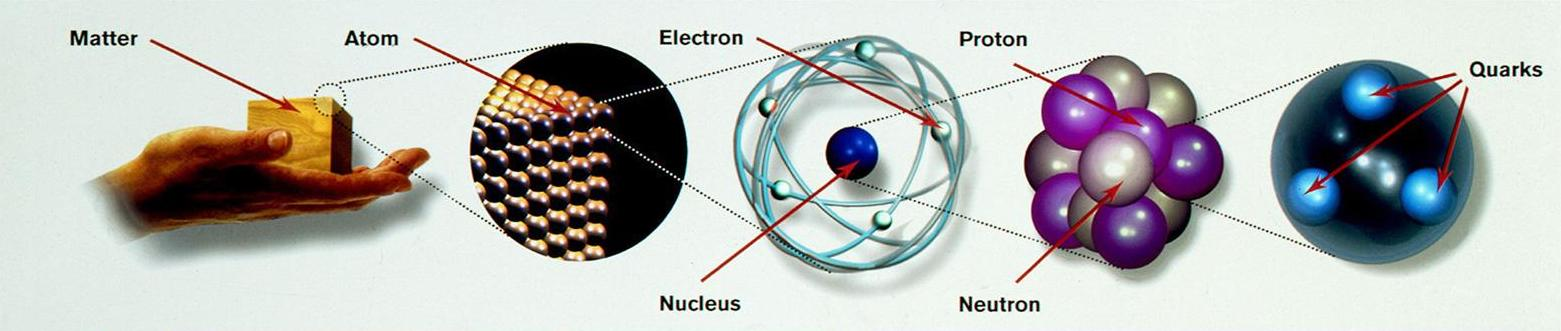
\includegraphics[height=0.55\textheight, width=\linewidth, keepaspectratio]{cmscern.jpeg}\\
      {\scriptsize Atoms are made of electrons and quarks (credit: CMS--CERN)}
    \end{column}
    \begin{column}{0.48\textwidth}
      \centering
      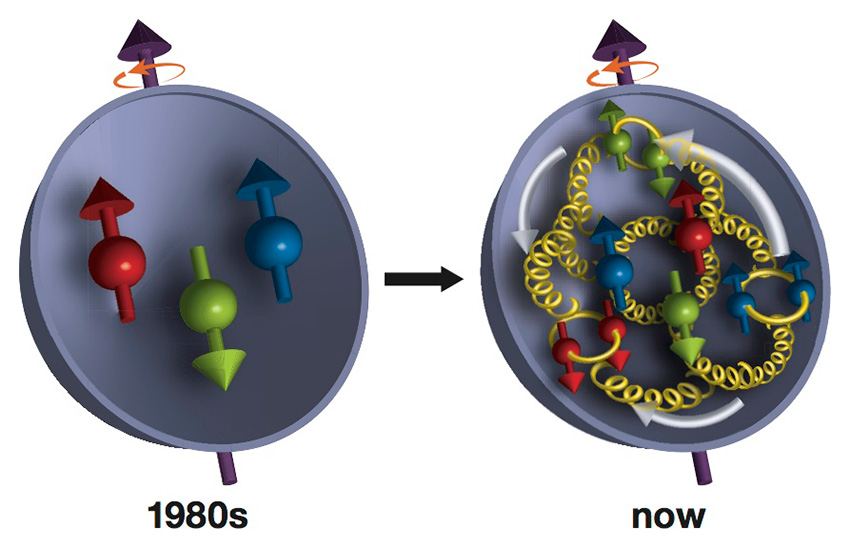
\includegraphics[height=0.55\textheight, width=\linewidth, keepaspectratio]{nucleon-large.jpg}\\
      {\scriptsize Internal structure of hadrons: quarks and gluons (credit: BNL)}
    \end{column}
  \end{columns}
\end{frame}

% Slide 8
\begin{frame}{QCD: Quantum Chromodynamics}
  The QCD Lagrangian density is built from two types of fields:
  \begin{itemize}
    \item spin-$\frac12$ Dirac fields (quarks) $\psi^{i}_{f}$: color $i = 1, 2, 3 = N_c$, flavor $f=u,d,s,c,b,t$;
    \item massless spin-1 vector fields (gluons) $A_{\mu}^{a}$: color $a=1,\ldots,8=N_c^{2}-1$, with local $SU(3)$ color gauge symmetry.
  \end{itemize}
  \[ \boxed{\mathcal{L}_{QCD}=-\frac{1}{4}F^{a}_{\mu\nu}F^{a\,\mu\nu}+\sum_{f}\bar{\psi}_{f}\big(i\gamma^{\mu}D_{\mu}-m_{f}\big)\psi_{f}} \]
  \begin{itemize}
    \item Field strength: $F^a_{\mu\nu}=\partial_{\mu}A^a_{\nu}-\partial_{\nu}A^a_{\mu}+g f^{abc}A^b_{\mu}A^c_{\nu}$
    \item Covariant derivative: $D_{\mu}=\partial_{\mu}-igA^a_{\mu}t^{a}$, \quad $[t^{a},t^{b}]=if^{abc}t^{c}$
    \item Asymptotic freedom at short distances; confinement at hadronic scales $\Rightarrow$ hadron structure is non-perturbative.
  \end{itemize}
\end{frame}
